\section{Containers structure and use}
\begin{frame}
Container technology is not very old \newline
\vspace{0.5cm}
The most famous: 
\includegraphics[width=0.2\textwidth]{docker_logo2.png} \newline
\vspace{0.5cm}
Solomon Hykes was inspirated by container port in the world travel \newline
\vspace{0.5cm}
\centering{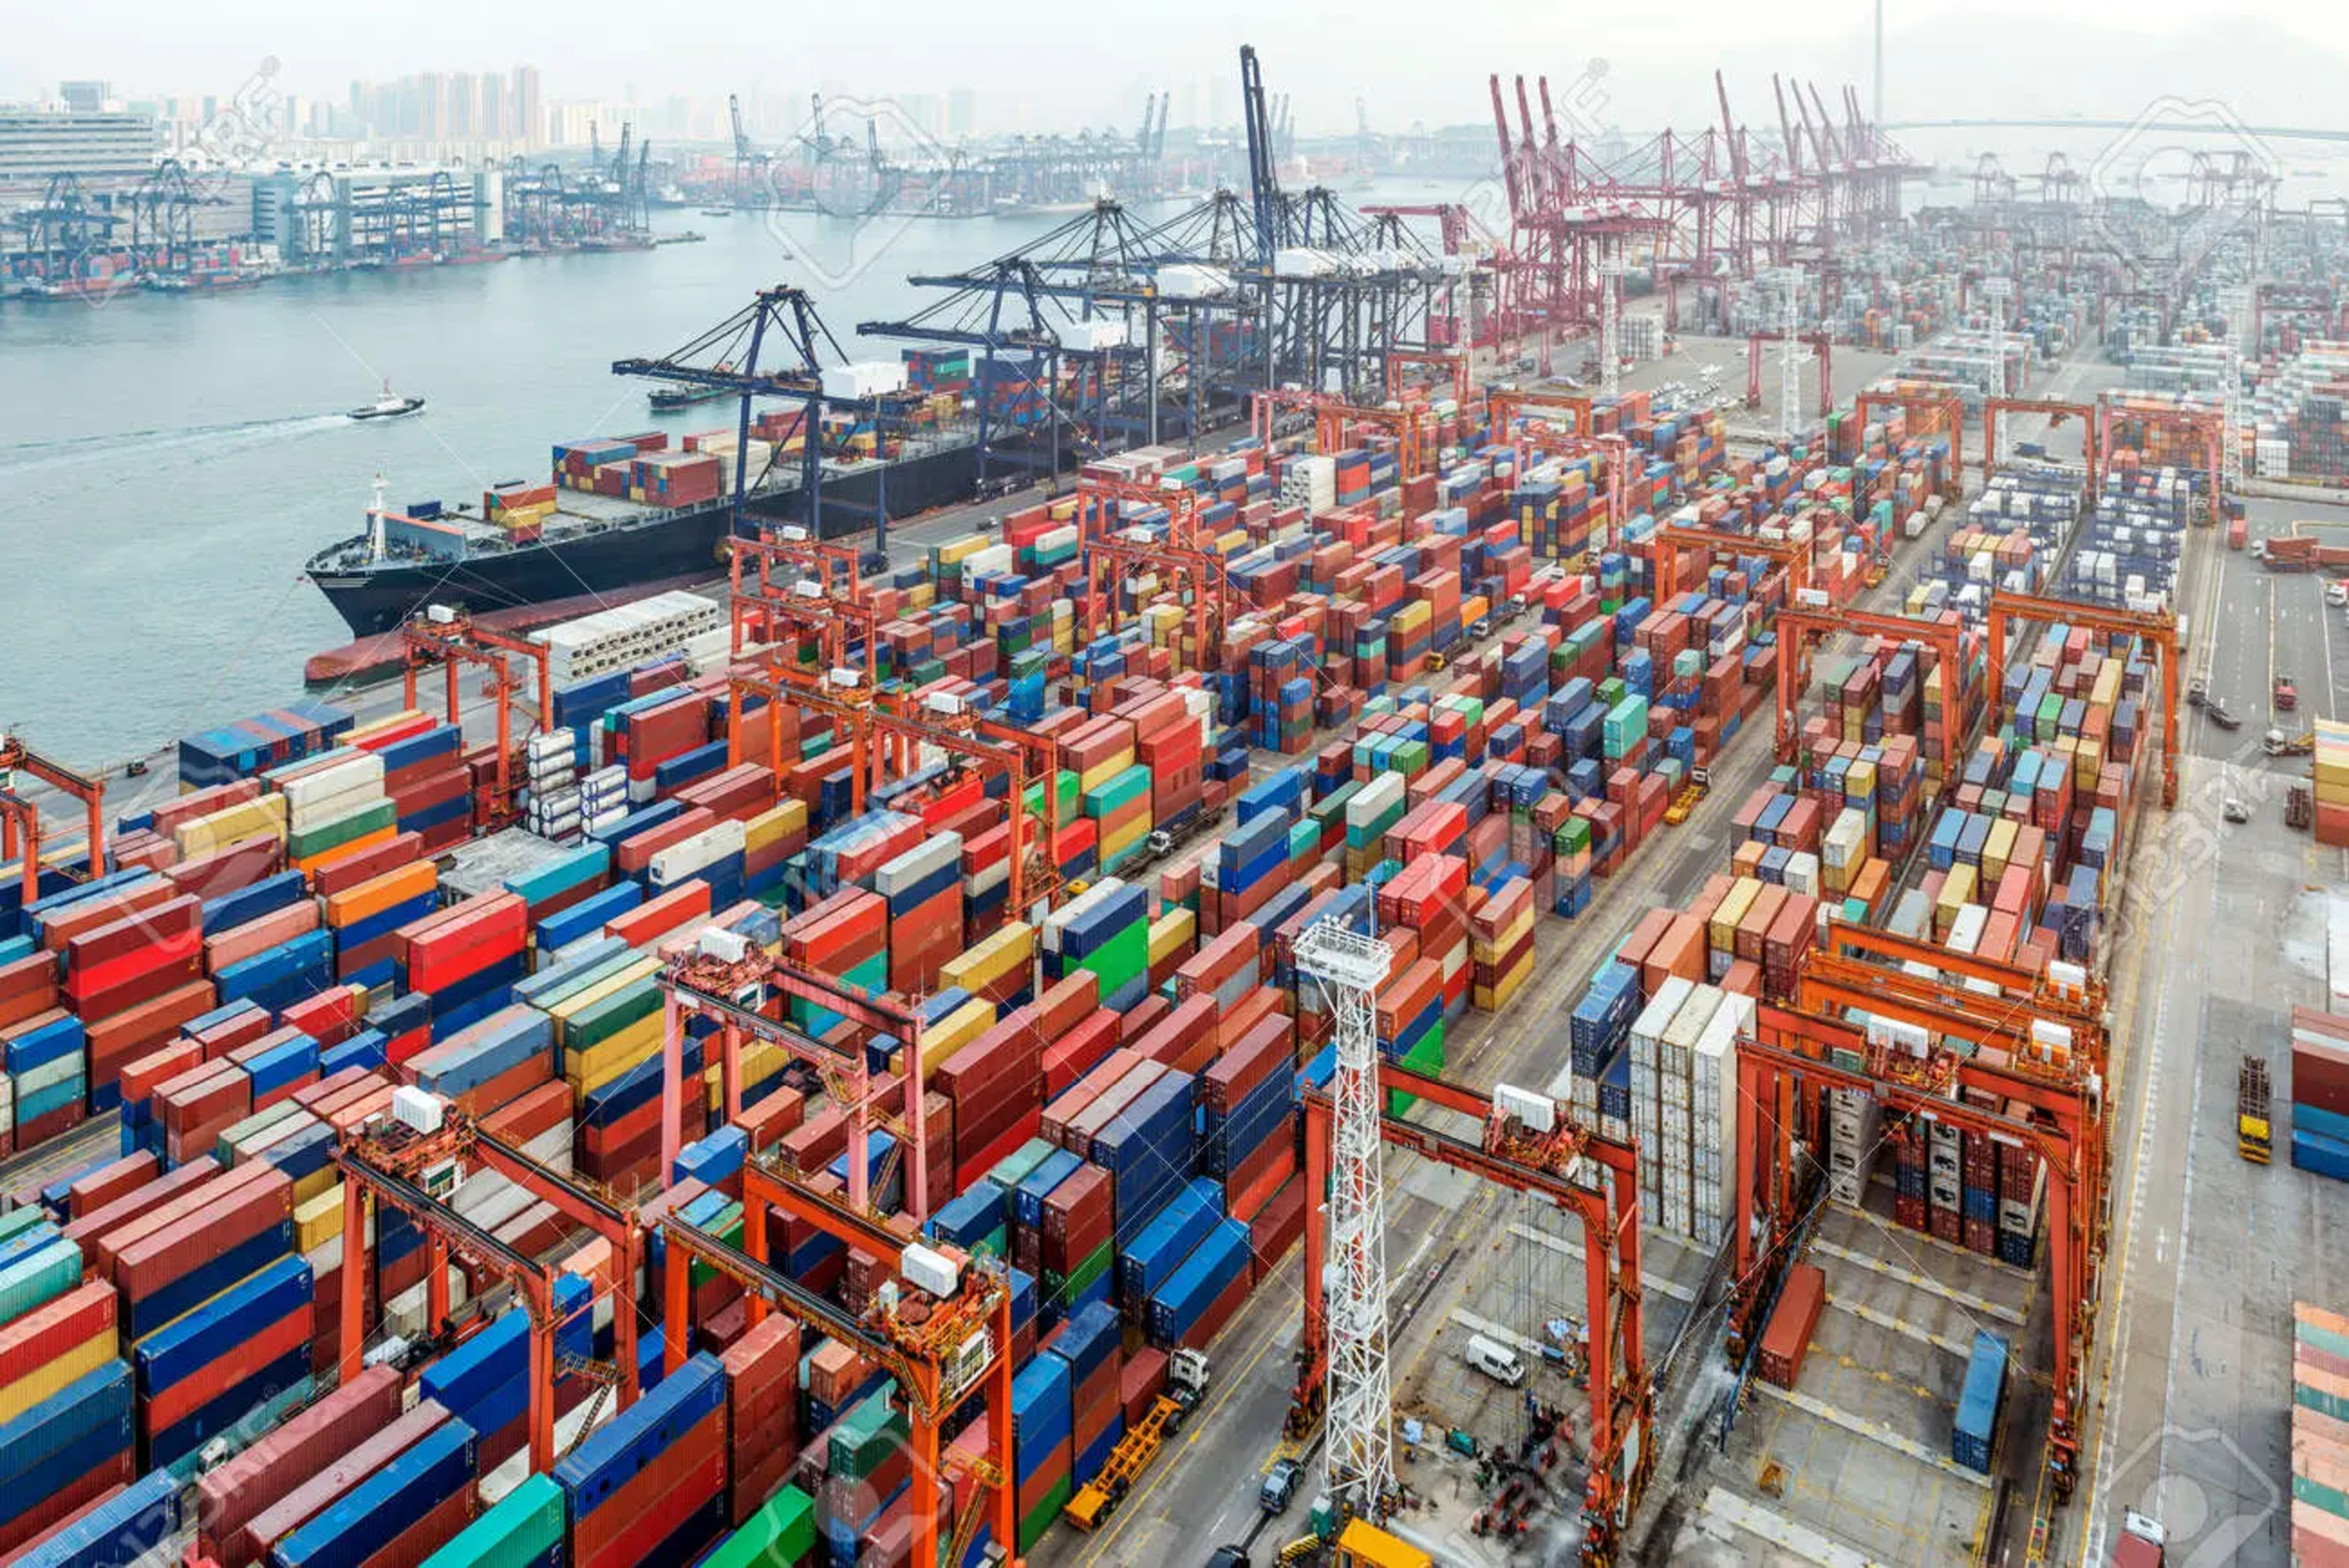
\includegraphics[width=0.4\textwidth]{container_port.pdf}} \newline
Docker is an open source project, a community and a private company 
\end{frame}

\begin{frame}
\begin{itemize}
\item Born in 2010
\item First public release in 2013
\item V 1.0 in 2014
\item Open source and free
\item Packaged to Ubuntu in 2014 (V14.04)
\end{itemize}
\end{frame}

\subsection{Docker}{Term definitions}
\begin{frame}
\begin{columns}
\column{.48\textwidth}
\begin{itemize}[<1->]
\item Docker image --> "snapshot" immutable file
	\begin{itemize}
	\item Set of libraries, functions
	\item Static state
	\item Online Store or share
	\item Automatically build
	\end{itemize}
\end{itemize}
\column{.48\textwidth}
\begin{itemize}[<2->]
\item Docker container --> instance of an image
	\begin{itemize}
	\item Result of the image activation
	\item Can be modified
	\item Can be tunred into an image
	\item 1 image --> multiple containers 
	\end{itemize}
\end{itemize} 
\end{columns}
\end{frame}

\begin{frame}{Docker architecture}
client-server architecture \\
\centering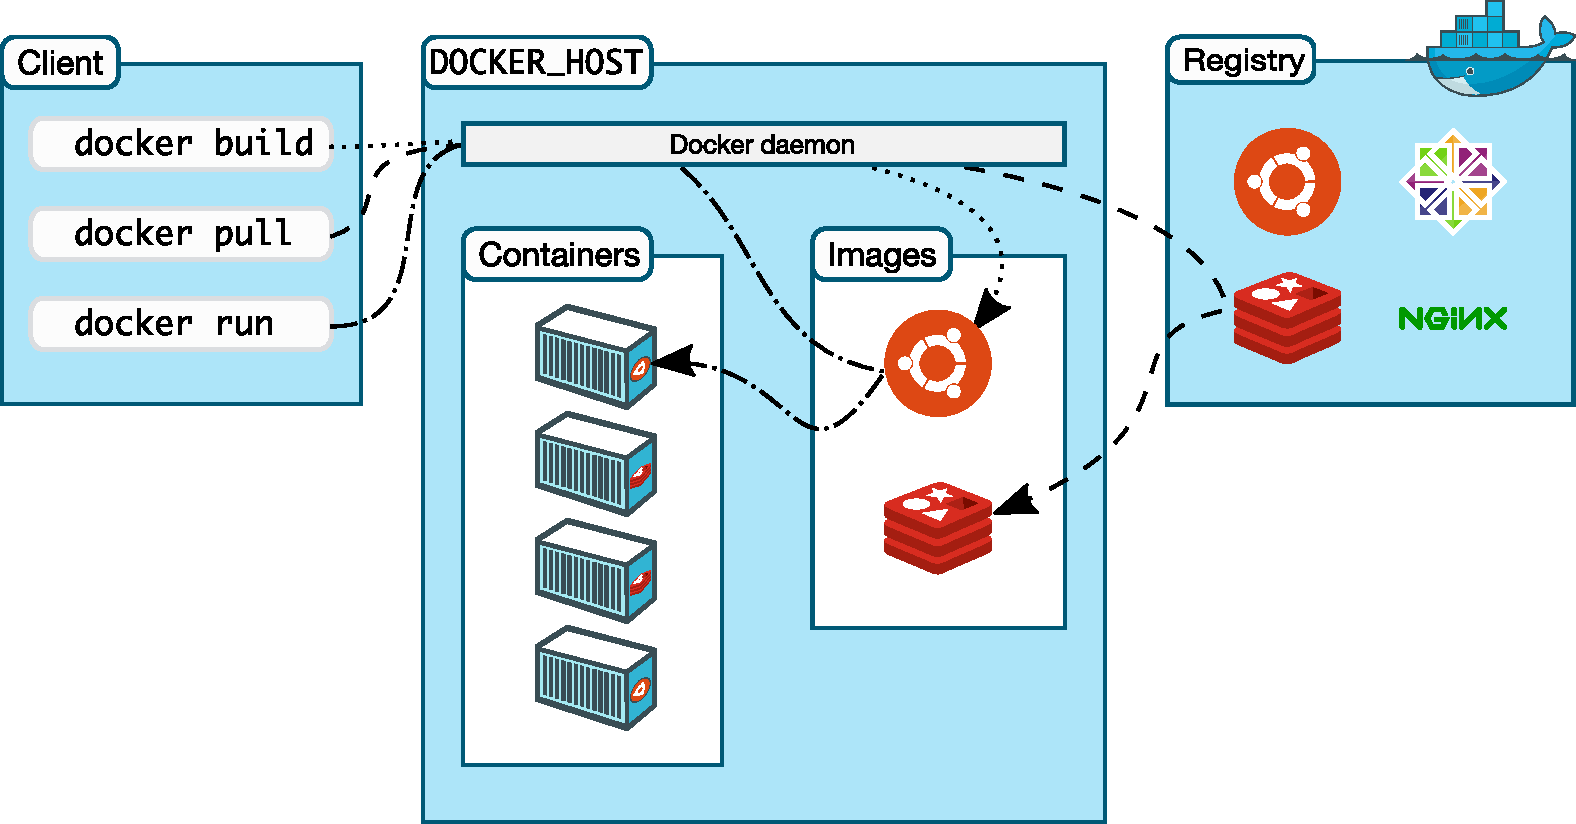
\includegraphics[width=0.8\textwidth]{docker_arch_3.pdf}
\end{frame}

\begin{frame}[fragile]{Docker client}
\begin{enumerate}
\item<1-> Client to interact with Docker
\item<2-> Client talk to the daemons (Docker background programs)
\begin{block}{Client}
\begin{verbatim}
$ docker build [path][url] 
  docker build https://github.com/docker/rootfs.git#container:docker
$ docker pull [image_name]
  docker pull biocontainers/samtools
$ docker run [image_name]
  docker run biocontainers/samtools
\end{verbatim}
\end{block}
\end{enumerate}

\begin{center}
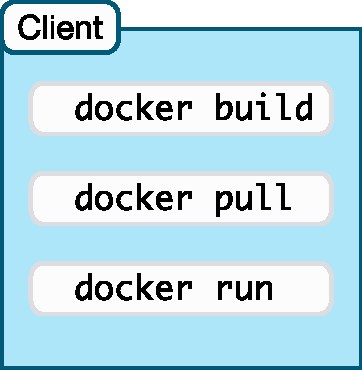
\includegraphics[width=0.15\textwidth]{docker_arch_1.pdf}
\end{center}
\end{frame}

\begin{frame}[<+->]{Docker daemon}
\begin{enumerate}
\item Listen client requests
\item Manage Dockers images, containers...
\end{enumerate}
\centering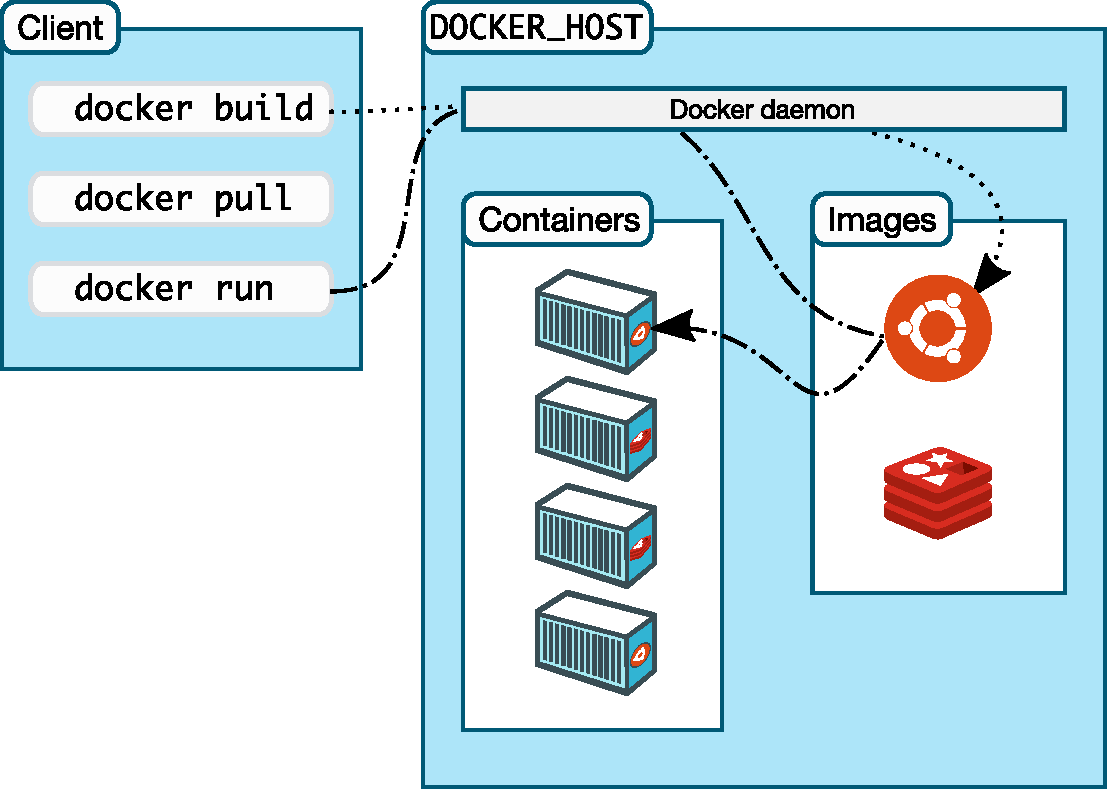
\includegraphics[width=0.6\textwidth]{docker_arch_2.pdf}
\end{frame}

\begin{frame}[<+->]{Docker registries}
\begin{enumerate}
\item Store Docker images
\item Docker hub is a public registry
\item You can run your own registry
\end{enumerate}
\onslide<2->{\centering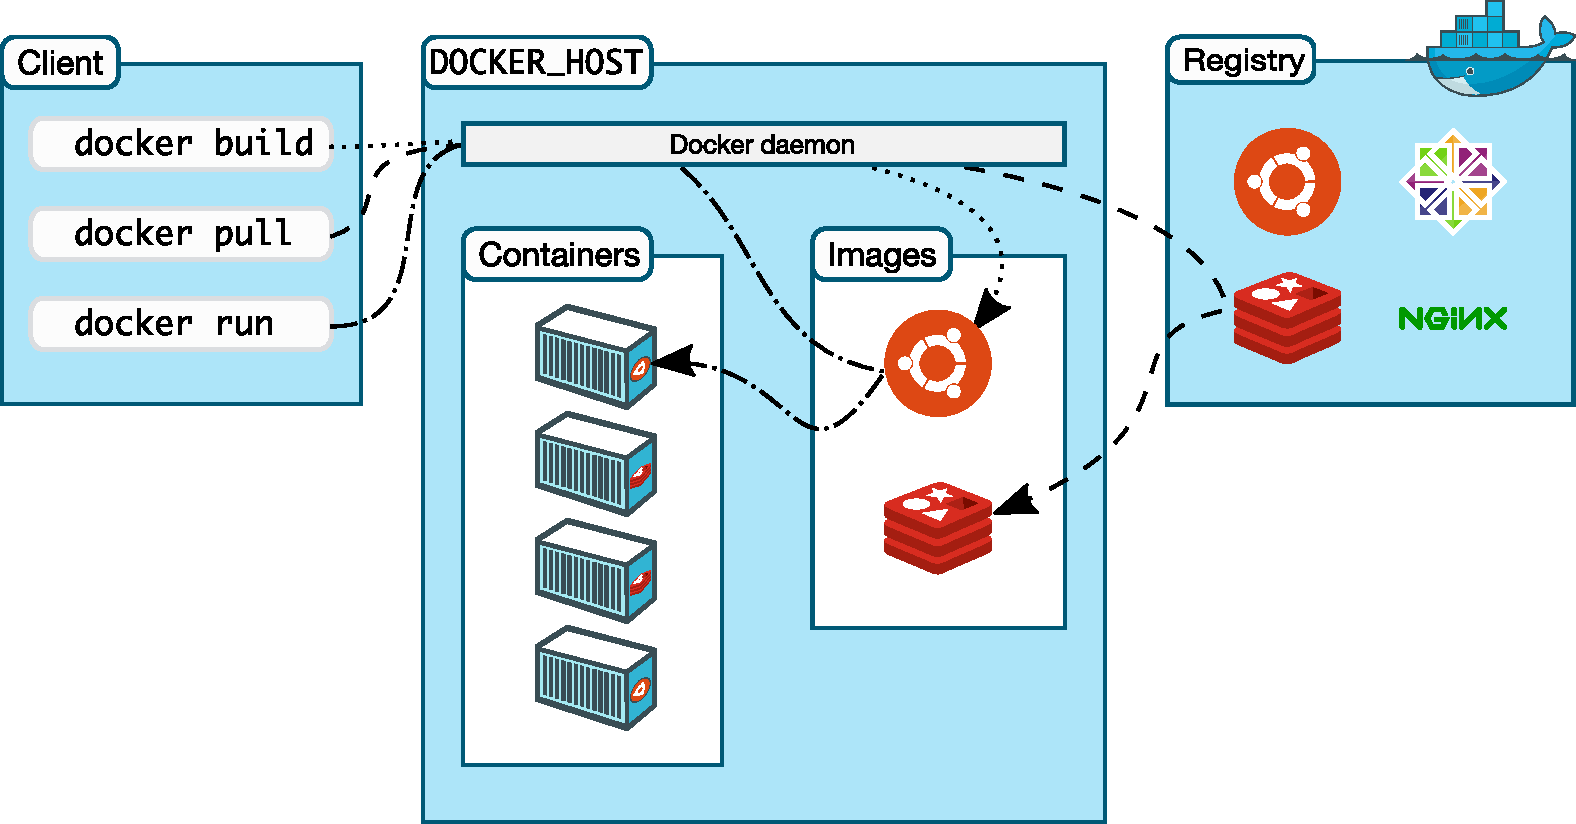
\includegraphics[width=0.75\textwidth]{docker_arch_3.pdf}}
\begin{textblock*}{10cm}(1cm,2cm)
\only<1>{\centering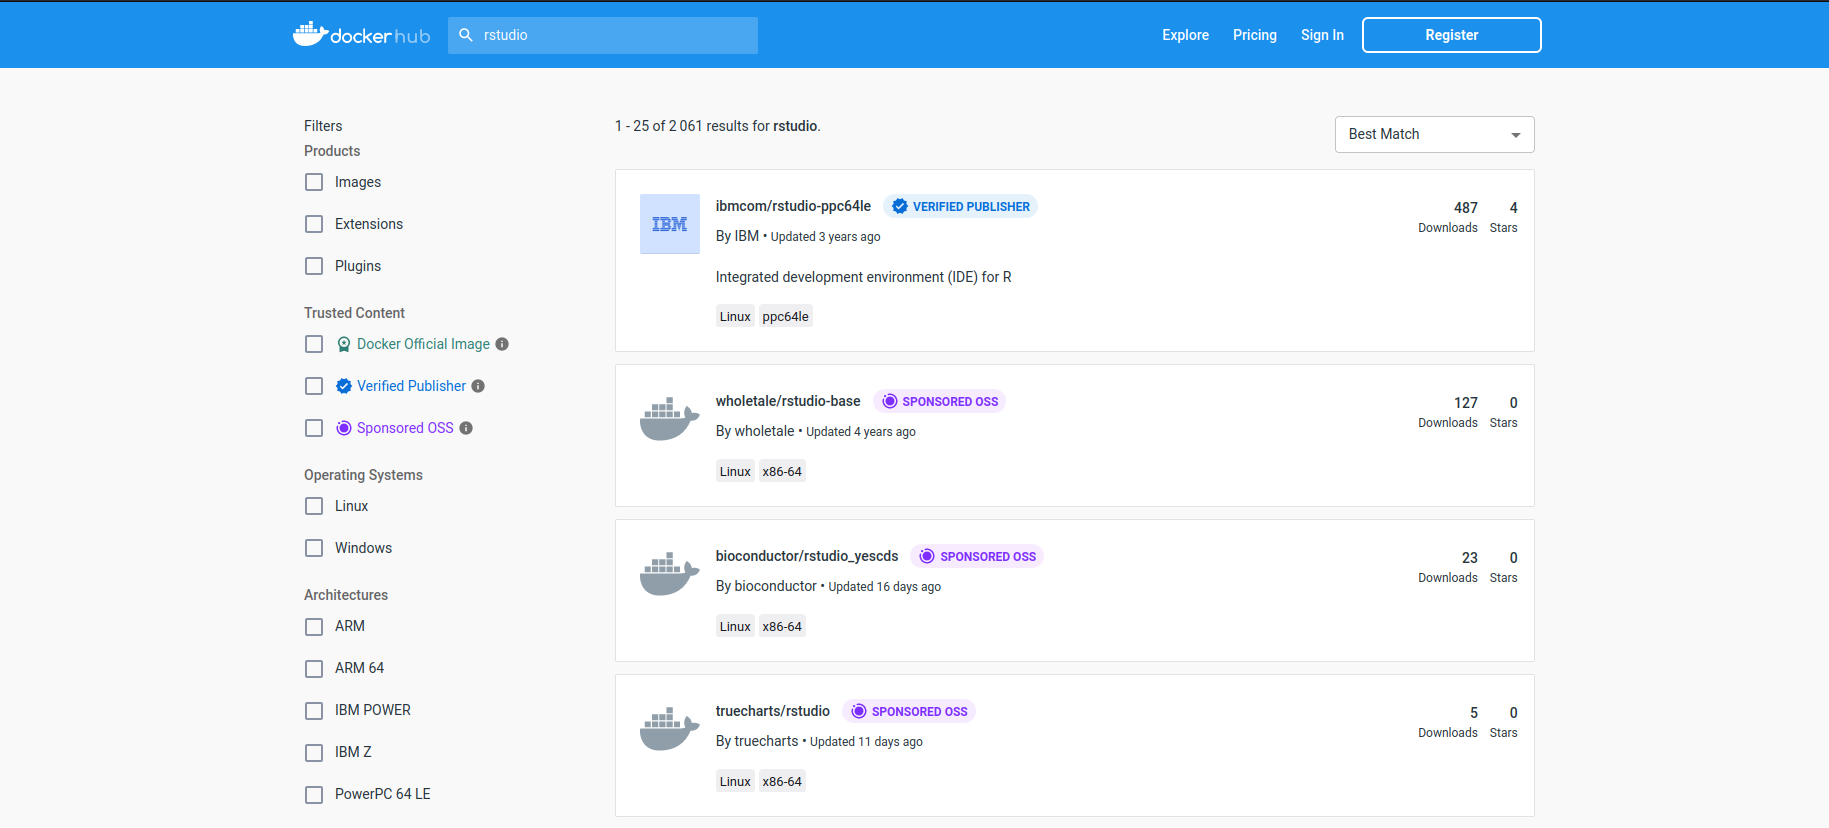
\includegraphics[width=1.4\textwidth]{docker_hub.png}}
\end{textblock*}
\end{frame}

\begin{frame}[fragile]{Image layers}
Focus on image building
\begin{itemize}[<+->]
\item Layers building
\item Several layers to one image
\end{itemize}
\end{frame}

\begin{frame}[fragile]{Image layers}
Focus on image building
\begin{itemize}
\item Layers building
\item Several layers to one image
\item Some layers shared by images when pulling
\item Lightheight the download and use of image on you computer
\end{itemize}
\begin{verbatim}
$ docker pull debian
Using default tag: latest
latest: Pulling from library/debian
fdd5d7827f33: Pull complete
a3ed95caeb02: Pull complete
Digest: sha256:e7d38b3517548a1c71e41bffe9c8ae6d6d29546ce46bf62159837aad072c90aa
Status: Downloaded newer image for debian:latest
\end{verbatim}
\end{frame}

\begin{frame}[fragile]{Pull me Hello world !}
\begin{itemize}
\item Try and pull your first image from docker hub
\begin{verbatim}
$ docker pull [path/url/docker_name]

$ docker pull hello-world
Using default tag: latest
latest: Pulling from library/hello-world
2db29710123e: Already exists 
Digest: sha256:63421b18c1443a9a85139225293fae7541fb40b7832d9deff80b6a9a75ce3604
Status: Downloaded newer image for hello-world:latest
docker.io/library/hello-world:latest

\end{verbatim}
\end{itemize}
\end{frame}

\begin{frame}[fragile]{Pull me Hello world !}
\begin{itemize}
\item Now run the hello-world image
\begin{verbatim}
$ docker image ls
REPOSITORY              TAG       IMAGE ID       CREATED         SIZE
hello-world             latest    feb5d9fea6a5   17 months ago   13.3kB
assembly_conda          latest    5ea57e9c4563   4 hours ago     2.99GB
assembly_raw            latest    dffe598c3a14   4 hours ago     990MB
condaforge/mambaforge   latest    8562647c2abf   12 days ago     393MB
ubuntu                  bionic    b89fba62bc15   2 weeks ago     63.1MB
\end{verbatim}
\end{itemize}
\end{frame}


\begin{frame}[fragile]{Pull me Hello world !}
\begin{itemize}
\item Now run the hello-world image
\begin{verbatim}
$ docker run[image_name/image_tag]
$ docker run hello-world
Hello from Docker!
This message shows that your installation appears to be working correctly.

To generate this message, Docker took the following steps:
 1. The Docker client contacted the Docker daemon.
 2. The Docker daemon pulled the "hello-world" image from the Docker Hub.
    (amd64)
 3. The Docker daemon created a new container from that image which runs the
    executable that produces the output you are currently reading.
 4. The Docker daemon streamed that output to the Docker client, which sent it
    to your terminal.
\end{verbatim}
\end{itemize}
\end{frame}

\begin{frame}{Build my own image}
\begin{block}{The basic recipe of Dockerfile}
\begin{itemize}
\item \textbf{FROM} A basic framework (image) as a linux, microsoft for ex. 
\item \textbf{RUN} A command to install a tool
\end{itemize}
\end{block}
\end{frame}

\begin{frame}{Build my own image}
Some few docker specific commands
AJOUTER UN LIEN DOCKER POUR LE SITTTTTTEEEE
\newline
\newline
\centering
\begin{tabular}{ll}
Instruction & Description \\
\hline\hline
FROM & Image parente \\
MAINTAINER & Auteur \\
ARG & Variables passées comme paramètres à la construction de l'image \\
ENV & Variable d'environnement \\
LABEL & Ajout de métadonnées \\
VOLUME & Crée un point de montage \\
RUN & Commande(s) utilisée(s) pour construire l'image \\
ADD & (Ajoute un fichier dans l'image *ADD vs COPY) \\
COPY & Ajoute un fichier dans l'image \\
WORKDIR & Permet de changer le chemin courant \\
EXPOSE & Port(s) écouté(s) par le conteneur \\
USER & Nom d'utilisateur ou UID à utiliser \\
ONBUILD & Instructions exécutées lors de la construction d'images enfants \\
CMD & Exécuter une commande au démarrage du conteneur \\
\end{tabular}
\end{frame}

\begin{frame}[fragile]{Build my own image}{Dockerfile skeleton}
\begin{block}{The basic recipe of Dockerfile}
\begin{itemize}
\item \textbf{FROM} A basic framework (image) as a linux, microsoft for ex. 
\item \textbf{RUN} A command to install a tool
\end{itemize}
\end{block}
\begin{verbatim}
FROM ubuntu:bionic
ARG USER="Coco"
LABEL maintainer.email="coco@lasticot.fr"
RUN apt-get update
RUN echo "HELLO WORLD !"
\end{verbatim}
\end{frame}

\begin{frame}[fragile]{Build command}
\begin{verbatim}
AJOUTER UN SOUS TITRE POUR EXPLCICITE RLE CAS DE GITHUB
AJOUTER code gras pour les commandes
$ docker build [url/path] --tag [docker_name]
special case with github url like :
[url]\#[branch_name][file_path]
$ docker build https://github.com/mesocentre-clermont-auvergne/formation_fair.git \
\#main:/fair_encapsulation/fair_encapsulation_TP/fair_encapsulation_containers/fair_encapsulation_docker/docker_assembly_raw 
-t assembly_raw
\end{verbatim}
\end{frame}


\begin{frame}[fragile]{Export docker image}
\begin{verbatim}
$ docker save [image_name/ID] > [image_name].tar
\end{verbatim}
\end{frame}

\begin{frame}
\centering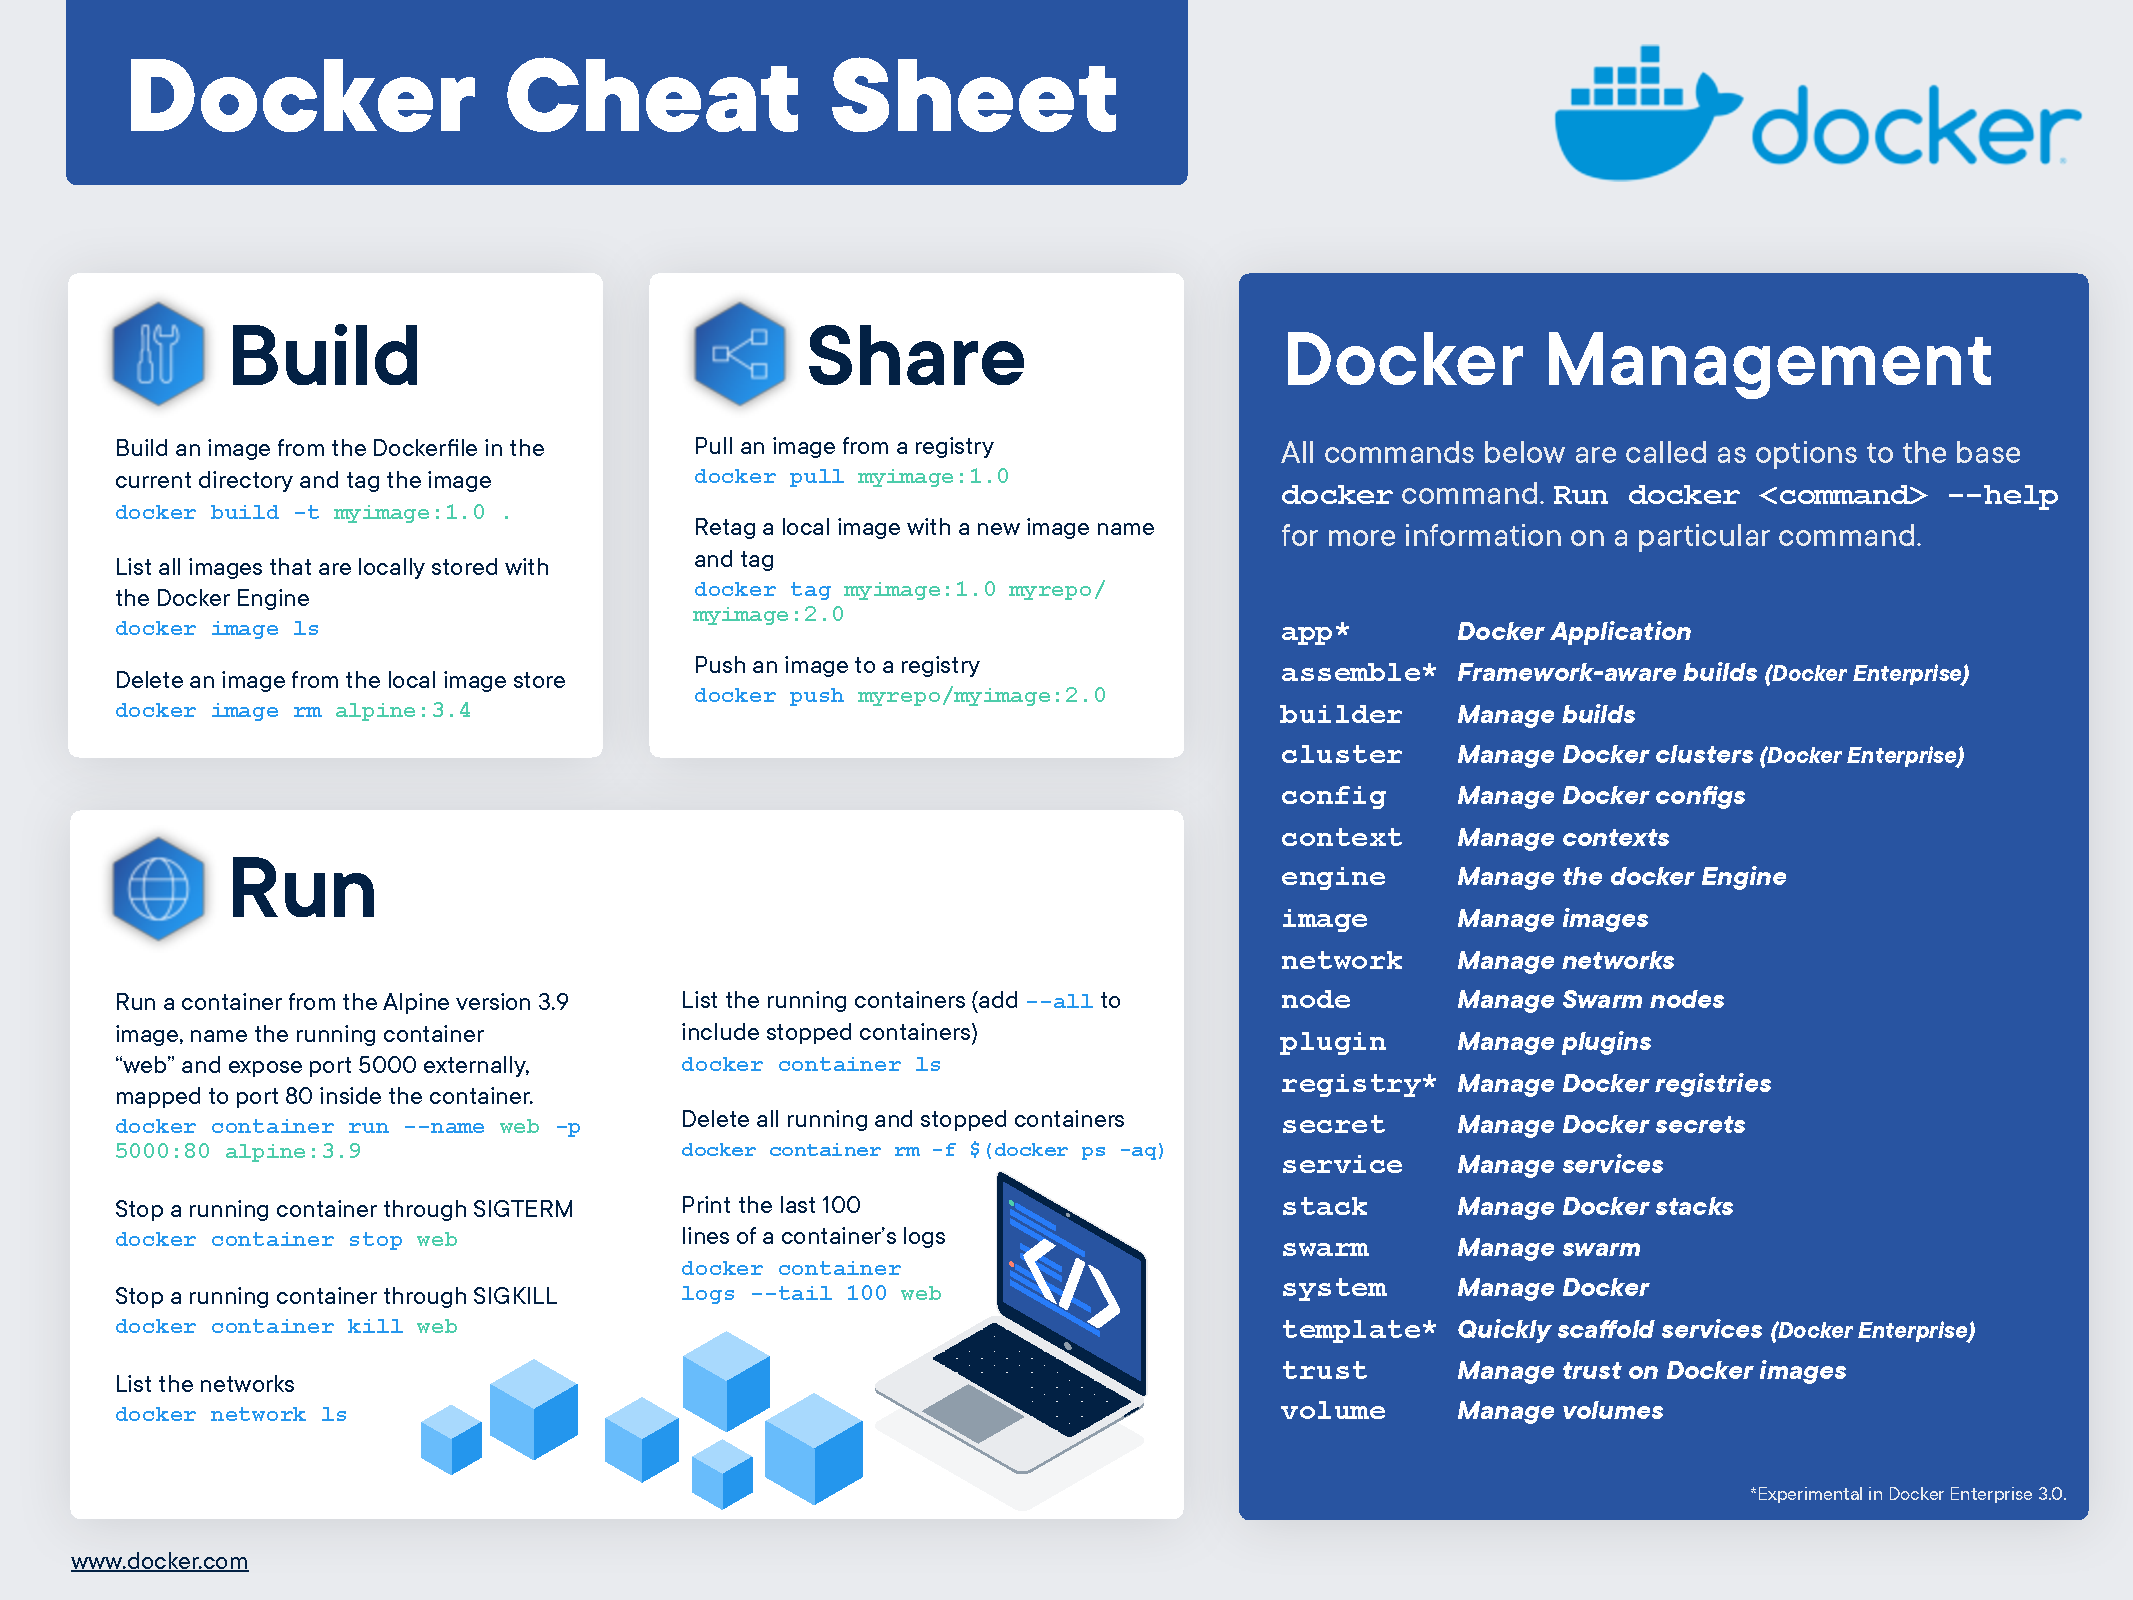
\includegraphics[width=0.9\textwidth]{docker-cheat-sheet.pdf}
\end{frame}

\begin{frame}
\centering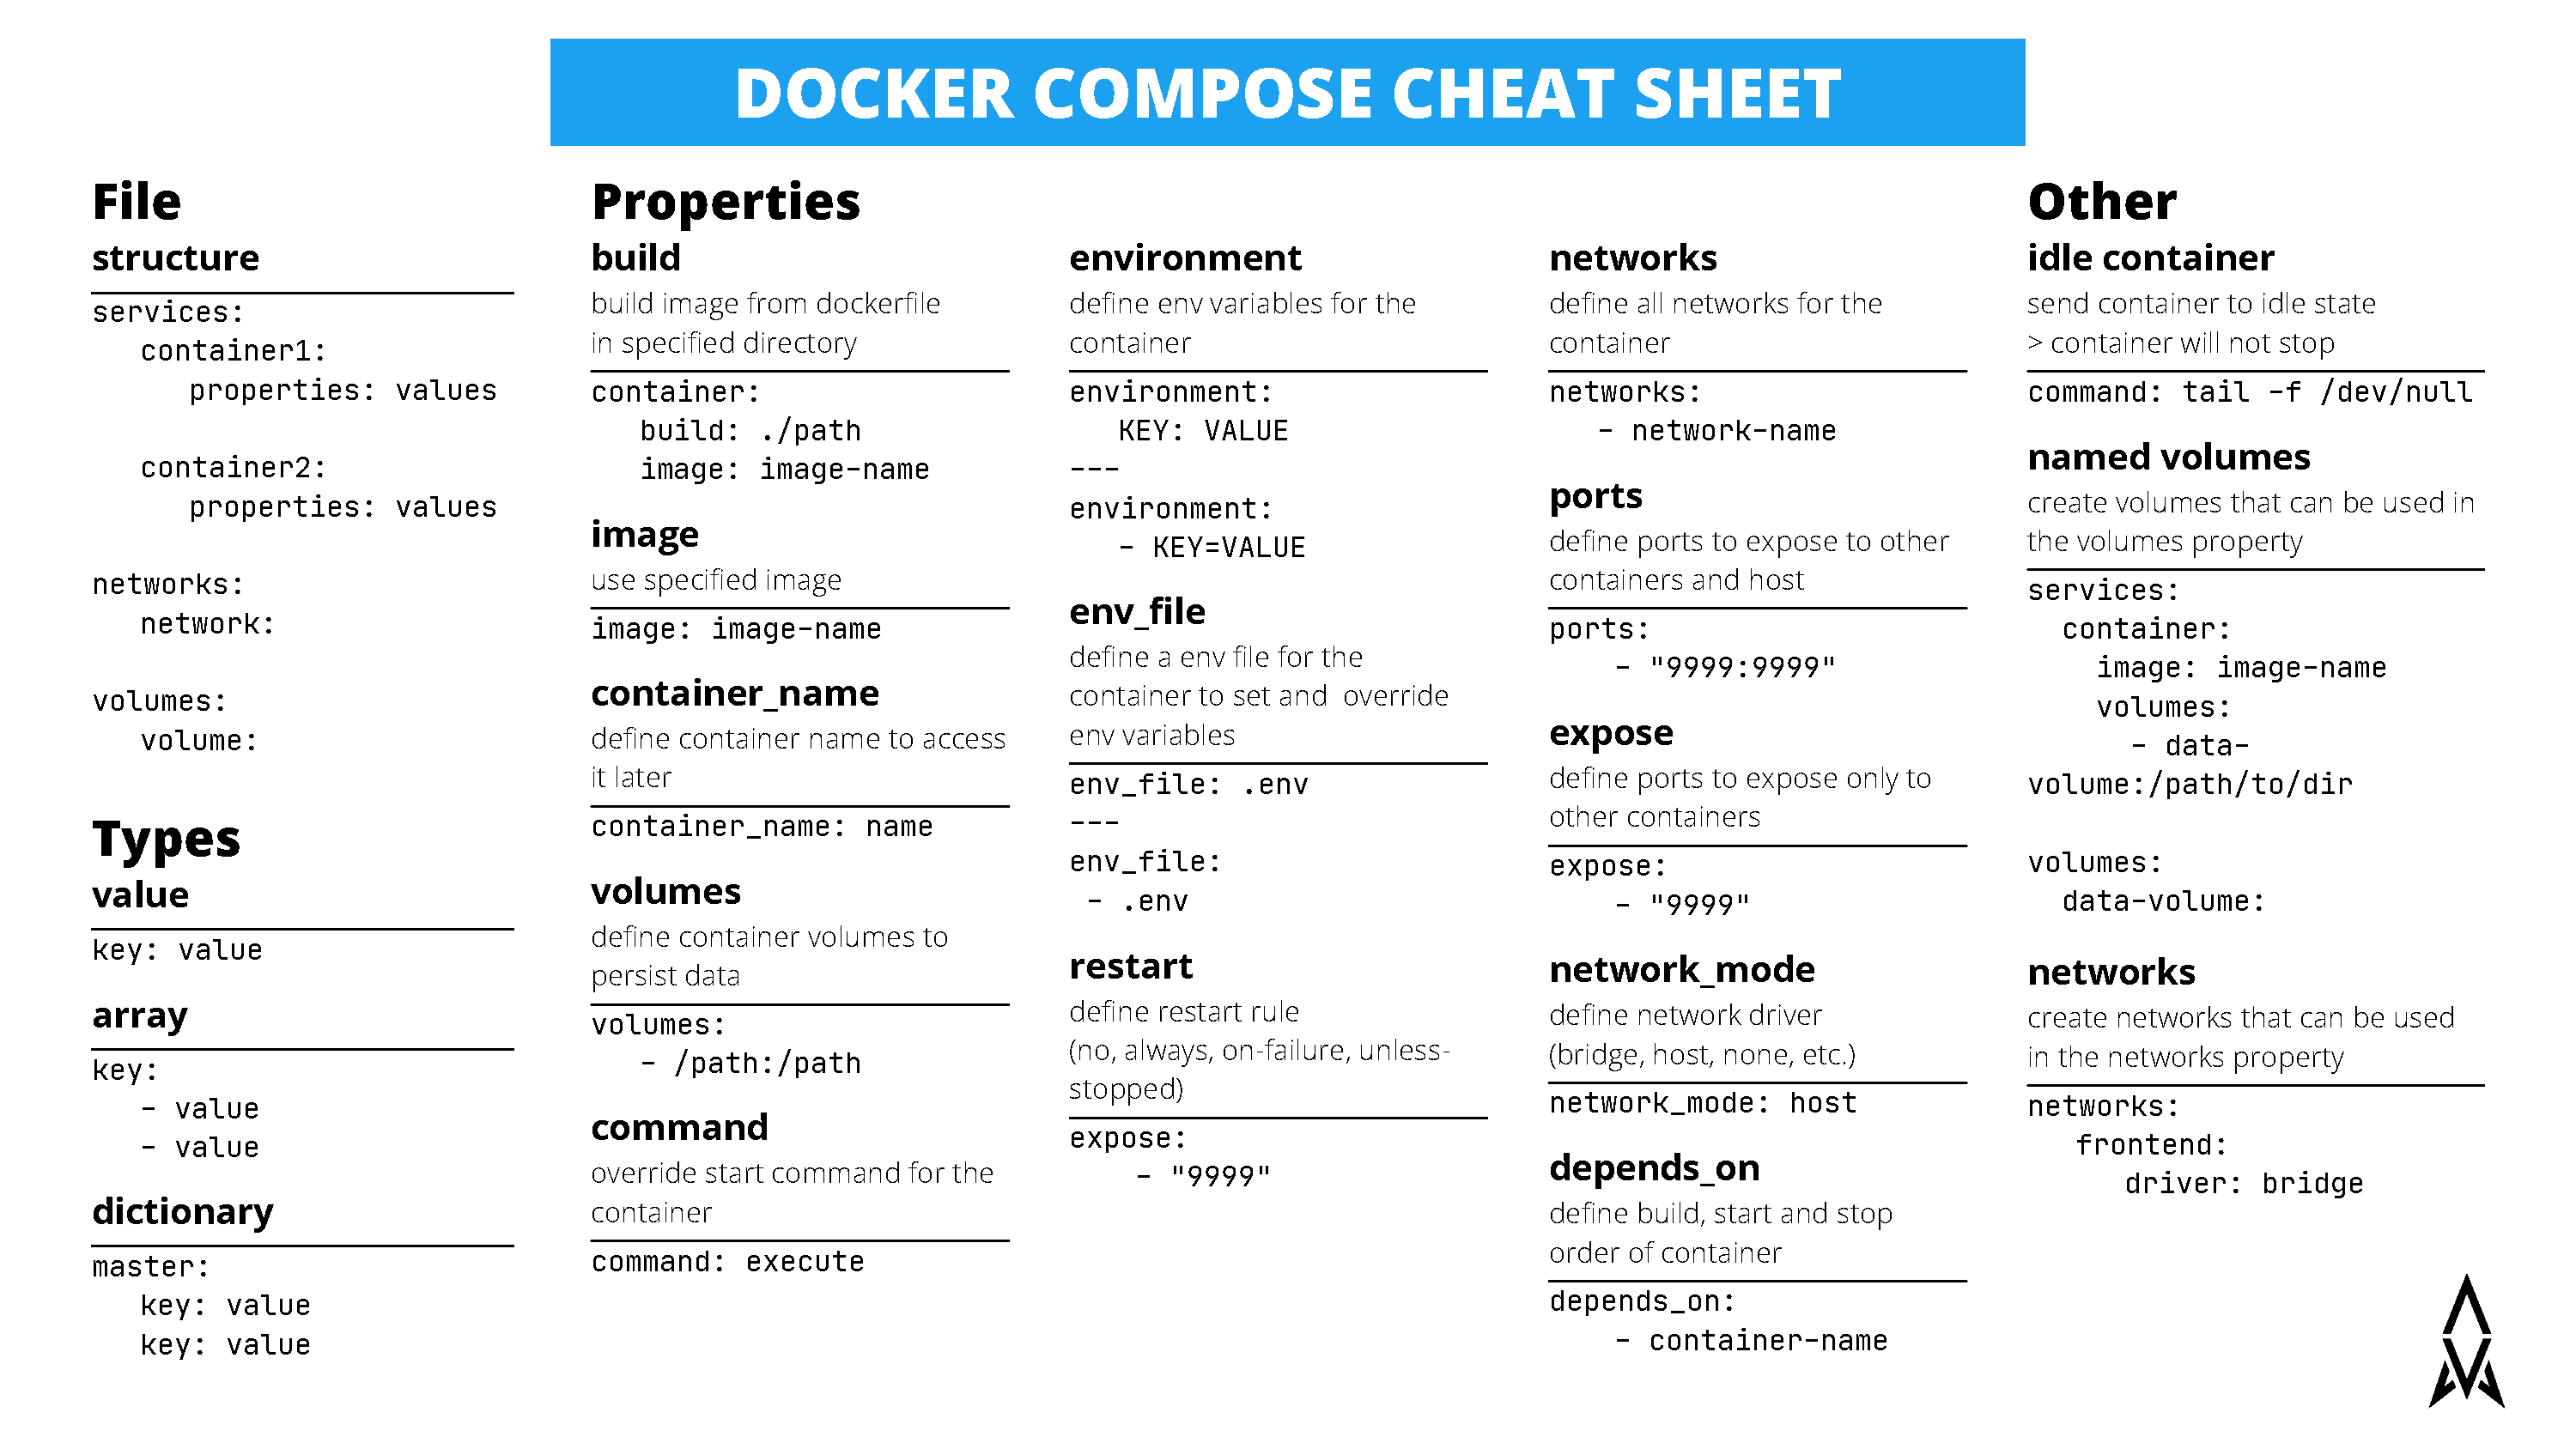
\includegraphics[width=0.9\textwidth]{docker-compose-cheat-sheet.pdf}
\end{frame}

\subsection{Singularity}
\begin{frame}[<+->]{Singularity history}
\begin{itemize}
\item Also a container manager as Docker
\item Open-source project
\item Release in 2015
\item Fork project in 2020 with now AppTainer (linux foundation) and SingularityCE
\item HPC compatible, no root write, integrate ressource managers (slurm)
\item Could use Docker images
\end{itemize}
\only<1>{\centering
\includegraphics[width=0.2\textwidth]{singularity_logo.pdf}}
\end{frame}

\begin{frame}[fragile]{Singularity commands}
\begin{columns}
\begin{column}{0.45\textwidth}
\begin{block}<1->{Docker command}
\begin{verbatim}
$ docker search [image_name]
$ docker pull [image_name]
$ docker run [image_name]
\end{verbatim}
\end{block}
\end{column}
\begin{column}{0.45\textwidth}
\begin{block}<2->{Singularity commands}
\begin{verbatim}
$ singularity search [image_name]
$ singularity pull [image_name]
$ singularity run [image_name]
\end{verbatim}
\end{block}
\end{column}
\end{columns}
\end{frame}

\begin{frame}[fragile]{Singularity and Docker}
\begin{block}{Singularity can use Docker images}
\begin{itemize}
\item from docker hub
\item from docker file
\end{itemize}
\end{block}
\begin{verbatim}
$ singularity build [new_image_name] docker-archive://[image_name].tar
$ singularity run [new_image_name]
$ singularity pull docker://debian:latest
INFO:    Converting OCI blobs to SIF format
INFO:    Starting build...
Getting image source signatures
Copying blob f606d8928ed3 done  
Copying config 0311b76201 done  
Writing manifest to image destination
Storing signatures
2022/10/06 10:50:41  info unpack layer: sha256:f606d8928ed378229f2460b94b504cca239fb906efc57acbdf9340bd298d5ddf
INFO:    Creating SIF file...
\end{verbatim}
\end{frame}

\begin{frame}{Singularity recipe}
\begin{tabular}{ll}
Bootstrap &  base you want to use (e.g., docker, debootstrap, shub) \\
From &  named container you want to use \\
\%help & help text to the user\\
\%setup & executed command on the host system outside the container\\
\%files & allow to copy file to the containers \\
\%labels & store metadata with your container, \\
\%environment & environment variables sourced at runtime \\
\%post setup & command of your container \\
\%runscript & started when container is running \\
\%test & command to test the image build \\
\end{tabular}
\end{frame}

\begin{frame}[fragile]{Singularity recipe}
\begin{verbatim}
Bootstrap: docker
From: ubuntu:bionic

%help
Help me. I'm in the container.
%labels
    Maintainer "coco l'asticot"
%environment
    VADER=badguy
    LUKE=goodguy
    export VADER LUKE
%post
    echo "Hello World !"
%runscript
    echo "Rooooar!"
\end{verbatim}
\end{frame}
